%! TEX program = pdflatex

\documentclass[oneside,solution]{karazin-control-assign}

\usepackage[utf8]{inputenc}
\usepackage[english,ukrainian]{babel}

\title{Домашня Робота}
\author{Захаров Дмитро}
\studentID{МП-31}
\instructor{Сморцова Т.І.}
\date{\today}
\duedate{23:59 31 березня, 2024}
\assignno{1}
\semester{Весняний семестр 2024}
\mainproblem{Варіант 3}

\begin{document}

\maketitle

% \startsolution[print]

\problem{Постійна матриця}

\hspace{20px}\textit{Умова.} Знайти керування, яке переводить точку $(0,0)$ в точку $\widetilde{\mathbf{x}} :=(\widetilde{x}_1,\widetilde{x}_2)$\footnote{Тут і далі форма $(x_1,\dots,x_n)$ позначає вектор $[x_1,\dots,x_n]^{\top}$.} в силу системи
\begin{equation}
    \begin{cases}
        \dot{x}_1 = 3x_1 - x_2 + u \\
        \dot{x}_2 = x_1 + x_2
    \end{cases}
\end{equation}
за час $[0,1]$. Виписати задачу Коші для знаходження траєкторії системи, за якою відбувається цей перехід.

\textit{Розв'язання.} Позначимо $\mathbf{x}(t) = (x_1(t),x_2(t))$, тоді наша система може бути записана у вигляді:
\begin{equation}
    \dot{\mathbf{x}} = \boldsymbol{A}\mathbf{x} + \boldsymbol{\beta}u,
\end{equation}
де ми ввели $\boldsymbol{A} = \begin{bmatrix}
    3 & -1 \\ 1 & 1
\end{bmatrix}, \;\boldsymbol{\beta} = (1,0)$. 

Перевіримо, чи є система повністю керованою за допомогою критерію Калмана. Для цього складаємо матрицю Калмана:
\begin{equation}
    \boldsymbol{K} \triangleq [\boldsymbol{\beta} \parallel \boldsymbol{A\beta}] = \begin{bmatrix}
        1 & 3\\
        0 & 1
    \end{bmatrix}
\end{equation}

Оскільки $\det\boldsymbol{K} = 1$, то $\text{rang}\,\boldsymbol{K} = 2$, отже система є повністю керованою. Це означає, що керування
\begin{equation}
    u(t) := \boldsymbol{\beta}^{\top}e^{-\boldsymbol{A}^{\top}t}\boldsymbol{N}^{-1}(0,1)e^{-\boldsymbol{A}}\widetilde{\mathbf{x}}
\end{equation}
є шуканим, де $\boldsymbol{N}(0,1)$ є інтегральною матрицею керованості:
\begin{equation}
    \boldsymbol{N}(0,1) \triangleq \int_0^1 \mathbf{w}(t)\mathbf{w}(t)^{\top}dt, \; \mathbf{w}(t) = \exp(-\boldsymbol{A}t)\boldsymbol{\beta}
\end{equation}

Далі рахуємо матричну експоненту:
\begin{equation}
    \exp(-\boldsymbol{A}t) = \begin{bmatrix}
        e^{-2t}(1-t) & e^{-2t}t \\
        -e^{-2t}t & e^{-2t}(1+t)
    \end{bmatrix}
\end{equation}

Отже, якщо помножимо на вектор $\boldsymbol{\beta}$:
\begin{equation}
    \mathbf{w}(t) = \begin{bmatrix}
        e^{-2t}(1-t) & e^{-2t}t \\
        -e^{-2t}t & e^{-2t}(1+t)
    \end{bmatrix}\begin{bmatrix}
        1 \\ 0
    \end{bmatrix} = \begin{bmatrix}
        e^{-2t}(1-t) \\
        -e^{-2t}t
    \end{bmatrix}
\end{equation}

Нарешті, це дозволяє нам порахувати інтегральну матрицю керованості:
\begin{equation}
    \boldsymbol{N}(0,1) = \int_0^1 \begin{bmatrix}
        e^{-4t}(1-t)^2 & -e^{-4t}(1-t)t \\
        -e^{-4t}(1-t)t & e^{-4t}t^2
    \end{bmatrix}dt
\end{equation}

Далі достатньо муторне інтегрування частинами по-елементно. В результаті маємо:
\begin{equation}
    \boldsymbol{N}(0,1) = \begin{bmatrix}
        \frac{1}{32}\left(5-\frac{1}{e^4}\right) & -\frac{3+e^4}{32e^4} \\
        -\frac{3+e^4}{32e^4} & \frac{1}{32}\left(1-\frac{13}{e^4}\right)
    \end{bmatrix}
\end{equation}

Далі беремо обернену матрицю:
\begin{equation}
    \boldsymbol{N}(0,1)^{-1} = \begin{bmatrix}
        \frac{8e^4(-13+e^4)}{1-18e^4+e^8} & \frac{8e^4(3+e^4)}{1-18e^4+e^8} \\
        \frac{8e^4(3+e^4)}{1-18e^4+e^8} & \frac{8e^4(-1+5e^4)}{1-18e^4+e^8}
    \end{bmatrix}
\end{equation}

Нарешті, підставляємо у вираз $u(t)$:
\begin{gather}
    u(t) = \mathbf{w}(t)^{\top}\boldsymbol{N}^{-1}(0,1)\exp(-\boldsymbol{A})\widetilde{\mathbf{x}} \nonumber \\
    = \begin{bmatrix}
        e^{-2t}(1-t) & e^{-2t}t
    \end{bmatrix}\begin{bmatrix}
        \frac{8e^4(-13+e^4)}{1-18e^4+e^8} & \frac{8e^4(3+e^4)}{1-18e^4+e^8} \\
        \frac{8e^4(3+e^4)}{1-18e^4+e^8} & \frac{8e^4(-1+5e^4)}{1-18e^4+e^8}
    \end{bmatrix}\begin{bmatrix}
        0 & e^{-2} \\ -e^{-2} & 2e^{-2}
    \end{bmatrix}\begin{bmatrix}
        \widetilde{x}_1 \\ \widetilde{x}_2
    \end{bmatrix}
\end{gather}

По-ітогу, результат має вигляд:
\begin{equation}
    u(t) = \langle\boldsymbol{\ell}(t),\widetilde{\mathbf{x}} \rangle,
\end{equation}
де
\begin{equation}
    \boldsymbol{\ell}(t) = \begin{bmatrix}
        -3+2t+(-1+6t)e^4 \\
        -7+6t+(3-14t)e^4
    \end{bmatrix}\frac{8e^{2(1-t)}}{1-18e^4+e^8}
\end{equation}

Отже, задача Коші виписується наступним чином:
\begin{equation}
    \dot{\mathbf{x}} = \boldsymbol{A}\mathbf{x} + \langle \boldsymbol{\ell}(t),\widetilde{\mathbf{x}}\rangle \boldsymbol{\beta}, \; \mathbf{x}(0) = \boldsymbol{\theta}, \; \mathbf{x}(1) = \widetilde{\mathbf{x}}
\end{equation}

Для перевірки, напишемо розв'язок цього рівняння у середовищі \textit{Wolfram Mathematica}. Код для цього має вигляд:
\begin{lstlisting}[language=Mathematica]
X1 = 0; Y1 = 3;
r1 = {X1, Y1};
k = 8*Exp[2-2t]/(1-18*Exp[4]+Exp[8]);
v[t_] = {-3+2t+Exp[4]*(-1+6t), -7+6t+Exp[4]*(3-14t)};
u[t_] = k*v[t].r1;
sol = DSolve[x'[t]==3*x[t]-y[t]+u[t] && y'[t]==x[t]+y[t] && x[0]==0 && y[0]==0, {x[t],y[t]}, t];
r[t_] = {sol[[1]][[1]][[2]], sol[[1]][[2]][[2]]};
ParametricPlot[r[t], {t, 0, 1}, PlotTheme -> "Scientific", 
 GridLines -> Automatic, PlotStyle -> {Thickness[0.01], Red}, 
 FrameLabel -> {"x1", "x2"}]
\end{lstlisting}

Тут у змінних $\mathtt{X1}$ та $\mathtt{Y1}$ ми кладемо $\widetilde{x}_1,\widetilde{x}_2$ відповідно і таким чином можемо отримати графік траєкторії на виході.

Графік на виході зображений на рисунку \ref{fig:problem-1}. Можемо дійсно бачити, що починаємо ми в $(0,0)$ і через час $t=1$ опиняємось у $(3,0)$ за допомогою системи з умови.
\begin{figure}
    \centering
    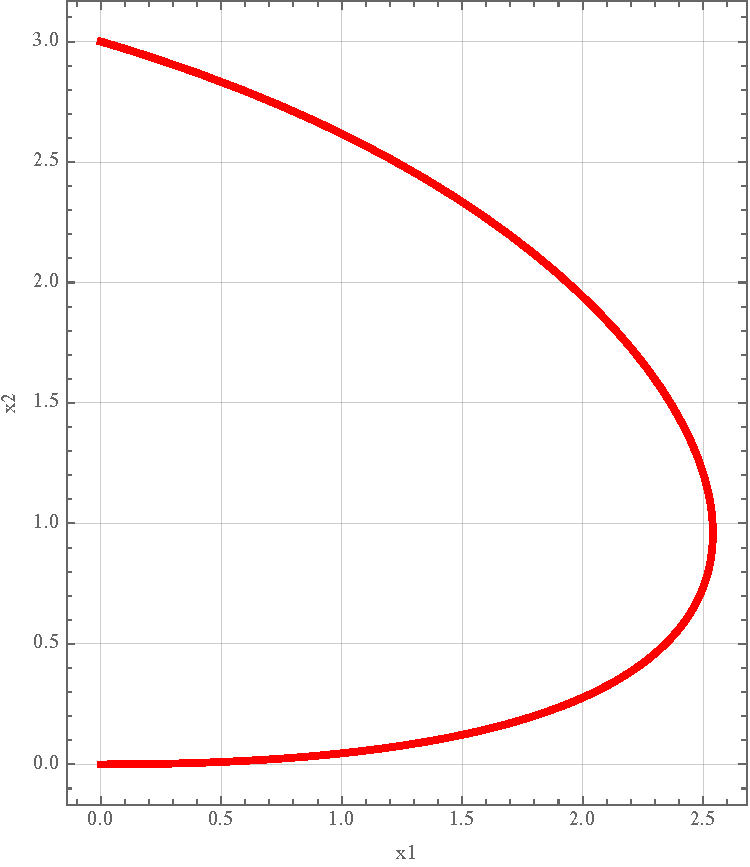
\includegraphics[width=0.5\textwidth]{plot_1.pdf}
    \caption{Графік траєкторії $\mathbf{x}(t)=(x_1(t),x_2(t))$ при $\widetilde{x}_1=0,\widetilde{x}_2=3$.}
    \label{fig:problem-1}
\end{figure}

\textbf{Відповідь.} $u(t) = \langle \boldsymbol{\ell}(t),\widetilde{\boldsymbol{x}}\rangle$, вектор $\boldsymbol{\ell}(t)$ дивись в розв'язанні.

\textit{Коментар.} Можна було дещо спростити життя, якщо б ми розглядали сімейство
\begin{equation}
    \boldsymbol{N}_f(0,1) \triangleq \int_0^1 f(t)e^{\boldsymbol{A}(1-t)}\boldsymbol{\beta}\boldsymbol{\beta}^{\top}e^{\boldsymbol{A}^{\top}(1-t)}dt,
\end{equation}
проте вирішив обрати найбільш механічний шлях :)

\problem{Змінна матриця}

\hspace{20px}\textit{Умова.} Знайти керування, яке переводить точку $(9,3)$ в точку $(0,0)$ в силу системи
\begin{equation}
    \begin{cases}
        \dot{x}_1 = 2x_2 + (t^2+5t)u \\
        \dot{x}_2 = \frac{1}{t+2}x_2 + (t+2)u
    \end{cases}
\end{equation}
за час $[0,3]$. Виписати задачу Коші для знаходження траєкторії системи, за якою відбувається цей перехід.

\textit{Розв'язання.} Якщо позначити $\mathbf{x}(t) := (x_1(t),x_2(t))$, то наша система може бути записана у вигляді
\begin{equation}
    \dot{\mathbf{x}} = \boldsymbol{A}(t)\mathbf{x} + \boldsymbol{\beta}(t)u,
\end{equation}
де ми позначили
\begin{equation}
    \boldsymbol{A}(t) = \begin{bmatrix}
        0 & 2 \\
        0 & \frac{1}{t+2}
    \end{bmatrix}, \; \boldsymbol{\beta}(t) = \begin{bmatrix}
        t(t+5) \\ t+2
    \end{bmatrix}
\end{equation}

Спочатку знайдемо фундаментальну матрицю $\boldsymbol{\Phi}(t)$, для цього потрібно розв'язати систему $\dot{\mathbf{x}} = \boldsymbol{A}(t)\mathbf{x}$ або:
\begin{equation}
    \begin{cases}
        \dot{x}_1 = 2x_2 \\
        \dot{x}_2 = \frac{1}{t+2}x_2
    \end{cases}
\end{equation}

Спочатку розв'яжемо друге рівняння. Маємо:
\begin{equation}
    \frac{dx_2}{dt} = \frac{x_2}{t+2} \implies \frac{dx_2}{x_2} = \frac{dt}{t+2} \implies \ln |x_2| = \ln (t+2) + C_1
\end{equation}

Звідси $x_2(t) = C_1(t+2)$. Підставляючи у друге, маємо:
\begin{equation}
    \frac{dx_1}{dt} = 2C_1(t+2) \implies dx_1 = 2C_1(t+2)dt \implies x_1 = C_1t^2 + 4C_1t + C_2 
\end{equation}

Отже, ми отримали, що
\begin{equation}
    \begin{bmatrix}
        x_1(t) \\ x_2(t)
    \end{bmatrix} = \begin{bmatrix}
        C_1t^2 + 4C_1t + C_2 \\
        C_1(t+2)
    \end{bmatrix} = \begin{bmatrix}
        t^2+4t & 1 \\ t+2 & 0
    \end{bmatrix}\begin{bmatrix}
        C_1 \\ C_2
    \end{bmatrix},
\end{equation}
звідки шукана фундаментальна матриця і обернена їй:
\begin{equation}
    \boldsymbol{\Phi}(t) = \begin{bmatrix}
        t^2 + 4t & 1 \\ t+2 & 0
    \end{bmatrix}, \; \boldsymbol{\Phi}^{-1}(t) = \begin{bmatrix}
        0 & \frac{1}{t+2} \\ 1 & -\frac{t^2+4t}{2+t}
    \end{bmatrix}
\end{equation}

Далі, знаходимо інтегральну матрицю керованості:
\begin{equation}
    \boldsymbol{N}(0,3) = \int_0^3 \boldsymbol{\Phi}^{-1}(t)\boldsymbol{\beta}(t)\boldsymbol{\beta}(t)^{\top}\boldsymbol{\Phi}^{-1}(t)^{\top}dt
\end{equation}

Для цього спочатку знайдемо наступний вектор:
\begin{equation}
    \mathbf{w}(t) = \boldsymbol{\Phi}^{-1}(t)\boldsymbol{\beta}(t) = \begin{bmatrix}
        0 & \frac{1}{t+2} \\ 1 & -\frac{t^2+4t}{2+t}
    \end{bmatrix}\begin{bmatrix}
        t(t+5) \\ t+2
    \end{bmatrix} = \begin{bmatrix}
        1 \\ t
    \end{bmatrix}
\end{equation}

Отримали несподівано простий вигляд. Отже,
\begin{equation}
    \boldsymbol{N}(0,3) = \int_0^3 \begin{bmatrix}
        1 & t \\ t & t^2
    \end{bmatrix}dt = \begin{bmatrix}
        3 & \frac{9}{2} \\ \frac{9}{2} & 9
    \end{bmatrix} \implies \boldsymbol{N}^{-1}(0,3) = \begin{bmatrix}
        \frac{4}{3} & -\frac{2}{3} \\ -\frac{2}{3} & \frac{4}{9}
    \end{bmatrix}
\end{equation}

Нарешті, керування можна записати у вигляді:
\begin{equation}
    u(t) = \mathbf{w}(t)^{\top}\boldsymbol{N}^{-1}(0,3)\left(\boldsymbol{\Phi}^{-1}(3)\mathbf{x}_1 - \boldsymbol{\Phi}^{-1}(0)\mathbf{x}_0\right)
\end{equation}

Оскільки $\mathbf{x}_1 = \boldsymbol{\theta}$, то вираз дещо спрощується:
\begin{equation}
    u(t) = -\mathbf{w}(t)^{\top}\boldsymbol{N}^{-1}(0,3)\boldsymbol{\Phi}^{-1}(0)\mathbf{x}_0
\end{equation}

Оскільки $\boldsymbol{\Phi}^{-1}(0)=\begin{bmatrix}
    0 & \frac{1}{2} \\ 1 & 0
\end{bmatrix}$, то остаточно
\begin{gather}
    u(t) = -\begin{bmatrix}
        1 & t
    \end{bmatrix}\begin{bmatrix}
        \frac{4}{3} & -\frac{2}{3} \\ -\frac{2}{3} & \frac{4}{9}
    \end{bmatrix}\begin{bmatrix}
        0 & \frac{1}{2} \\ 1 & 0
    \end{bmatrix}\begin{bmatrix}
        9 \\ 3
    \end{bmatrix} \nonumber \\
    = -\begin{bmatrix}
        1 & t
    \end{bmatrix}\begin{bmatrix}
        \frac{4}{3} & -\frac{2}{3} \\ -\frac{2}{3} & \frac{4}{9}
    \end{bmatrix}\begin{bmatrix}
        \frac{3}{2} \\ 9
    \end{bmatrix} \nonumber \\
    = -\begin{bmatrix}
        1 & t
    \end{bmatrix}\begin{bmatrix}
        -4 \\ 3
    \end{bmatrix} = \boxed{-3t+4}
\end{gather}

Отже, задача Коші має вигляд:
\begin{equation}
    \begin{cases}
        \dot{x}_1 = 2x_2 + (t^2+5t)(-3t+4) \\
        \dot{x}_2 = \frac{1}{t+2}x_2 + (t+2)(-3t+4)
    \end{cases}, \; x_1(0) = 9, \; x_2(0) = 3
\end{equation}

Знову перевіримо, що це дійсно розв'язок. Код у \textit{Wolfram Mathematica}:
\begin{lstlisting}[language=Mathematica]
u[t_] = 4-3t;
sol = DSolve[x'[t]==2y[t]+(t^2+5t)u[t] && y'[t]==y[t]/(t+2)+(t+2)u[t] && x[0]==9 && y[0]==3, {x[t], y[t]}, t];
r[t_] = {sol[[1]][[1]][[2]], sol[[1]][[2]][[2]]};
ParametricPlot[r[t], {t, 0, 3}, PlotTheme -> "Scientific", 
 GridLines -> Automatic, PlotStyle -> {Thickness[0.005], Red}, 
 FrameLabel -> {"x1", "x2"}]
\end{lstlisting}

На виході маємо рис. \ref{fig:problem-2}, що дійсно переводить точку $(9,3)$ у $(0,0)$.

\begin{figure}
    \centering
    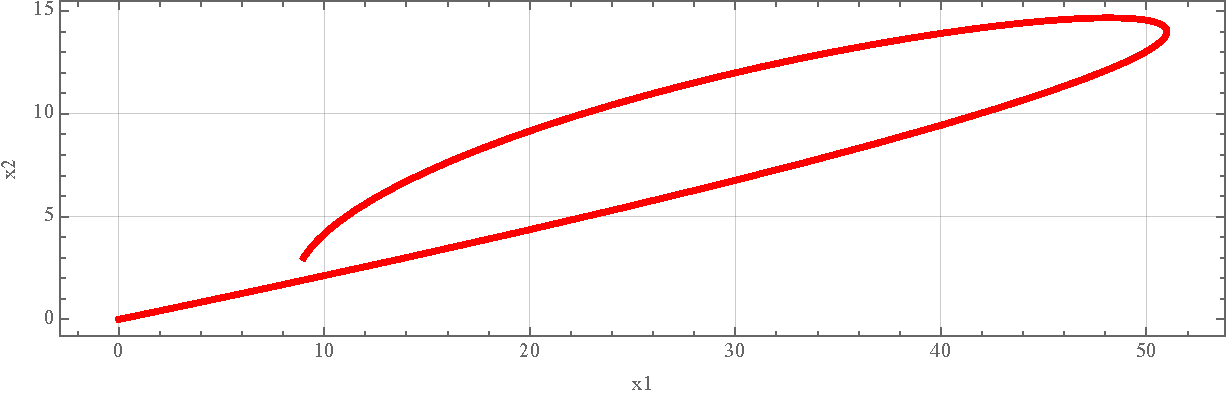
\includegraphics[width=0.9\textwidth]{plot_2.pdf}
    \caption{Графік траєкторії $\mathbf{x}(t)=(x_1(t),x_2(t))$ для $t \in [0,3]$.}
    \label{fig:problem-2}
\end{figure}

\textbf{Відповідь.} $u(t)=-3t+4$.

\end{document}
